% \documentclass[sigconf,anonymous,review,timestamp]{acmart}
% \documentclass[sigconf]{acmart}
\documentclass[acmtog]{acmart}
% \documentclass[acmtog,anonymous,review,timestamp]{acmart}
%%%%%%%%%%%%%%%%%%%%%%%%%%%%%%%%%%%%%%%%%%%%%%%%%%%%%%%%%%%%%%%%%%%%%%%%%%%

% From https://s2023.siggraph.org/program/technical-papers/ -- The submissions are required to adhere to the following length constraints: Papers must be no longer than 7 pages excluding references and figures-only pages. There is no limit on the length of the reference section. Each paper can have at most two figures-only pages, placed at the end of the submission, after references. Authors can also include as many figures as they wish within the core 7 pages. Papers should not include appendices in the main document.
%%%%%%%%%%%%%%%%%%%%%%%%%%%%%%%%%%%%%%%%%%%%%%%%%%%%%%%%%%%%%%%%%%%%%%%%%%%

%% Rights management information.  This information is sent to you
%% when you complete the rights form.  These commands have SAMPLE
%% values in them; it is your responsibility as an author to replace
%% the commands and values with those provided to you when you
%% complete the rights form.
\setcopyright{acmcopyright}
\copyrightyear{2023}
\acmYear{2023}
\acmDOI{XXXXXXX.XXXXXXX}

%% These commands are for a PROCEEDINGS abstract or paper.
\acmConference[Conference acronym 'XX]{Conference title}{January 01--02,
  1900}{Someplace, NY}
\acmPrice{15.00}
\acmISBN{978-1-4503-XXXX-X/18/06}

%%
%% Submission ID.
%% Use this when submitting an article to a sponsored event. You'll
%% receive a unique submission ID from the organizers of the event,
%% and this ID should be used as the parameter to this command.
\acmSubmissionID{123-A56-BU3}

%%
%% The majority of ACM publications use numbered citations and
%% references.  The command \citestyle{authoryear} switches to the
%% "author year" style.
%%
%% If you are preparing content for an event
%% sponsored by ACM SIGGRAPH, you must use the "author year" style of
%% citations and references.
%% Uncommenting
%% the next command will enable that style.
\citestyle{acmauthoryear}

%% To fix a margin violation bug, apparently due to poor hyphenation.
\hyphenation{Go-men-so-ro}

%% For introducing terms which have a special meaning in this work.
\newcommand{\jargon}[1]{\textit{#1}}

%% Stand-ins for software package names, anonymized for review.
% \newcommand{\texsyn}[0]{TexSyn}
\newcommand{\texsyn}[0]{pkgT}
\newcommand{\lazypredator}[0]{pkgE}
\newcommand{\predatoreye}[0]{pkgV}

%% for laying out a row of 4, 6, or 9 images
\newcommand{\igfour}[1]{\includegraphics[width=0.24\linewidth]{#1}}
\newcommand{\igsix}[1]{\includegraphics[width=0.16\linewidth]{#1}}
\newcommand{\ignine}[1]{\includegraphics[width=0.105\linewidth]{#1}}

\usepackage{changepage}  % http://ctan.org/pkg/changepage

\graphicspath{ {images/} {images/fcd5/} }

\begin{document}

\title{Coevolution of Camouflage}

%% Author
\author{Craig Reynolds}
\email{cwr@red3d.com}
\orcid{0000-0001-8203-712X}
\affiliation{%
  \institution{unaffiliated researcher}
  \country{USA}
}

\renewcommand{\shortauthors}{Craig Reynolds}

%%%%%%%%%%%%%%%%%%%%%%%%%%%%%%%%%%%%%%%%%%%%%%%%%%%%%%%%%%%%%%%%%%%%%%%%%%%

\begin{abstract}
    Camouflage in nature is thought to arise from competition between predator and prey. To survive, predators must find prey, and prey must avoid being found. This work simulates an abstract model of that adversarial relationship. It looks at \textit{crypsis} through evolving prey camouflage patterns (as color textures) in competition with evolving predator vision which learns to locate camouflaged prey. The environment for this 2D simulation is provided by a set of photographs, typically of natural scenes. This model is based on one evolving population of prey and another of predators. The mutual conflict between these populations appears to produce both effective camouflage and skilled predators. This simulation provides a method for creating camouflage patterns for arbitrary backgrounds, but more significantly, an open source \textit{artificial life} model for investigating aspects of camouflage evolution in nature. \textbf{(Note to reviewers: all source code and development notes will be posted online if paper is accepted. In this draft, modules are given anonymized names: \texsyn{}, \lazypredator{}, \predatoreye{}.)}
\end{abstract}

%%%%%%%%%%%%%%%%%%%%%%%%%%%%%%%%%%%%%%%%%%%%%%%%%%%%%%%%%%%%%%%%%%%%%%%%%%%

%%
%% Generate your CCSCML using http://dl.acm.org/ccs.cfm.
%%
\begin{CCSXML}
<ccs2012>
   <concept>
       <concept_id>10010147.10010341.10010349.10011810</concept_id>
       <concept_desc>Computing methodologies~Artificial life</concept_desc>
       <concept_significance>500</concept_significance>
       </concept>
   <concept>
       <concept_id>10010147.10010371.10010382.10010384</concept_id>
       <concept_desc>Computing methodologies~Texturing</concept_desc>
       <concept_significance>300</concept_significance>
       </concept>
   <concept>
       <concept_id>10010147.10010178.10010224</concept_id>
       <concept_desc>Computing methodologies~Computer vision</concept_desc>
       <concept_significance>300</concept_significance>
       </concept>
    <concept>
       <concept_id>10010147.10010178.10010224.10010245.10010246</concept_id>
       <concept_desc>Computing methodologies~Interest point and salient region detections</concept_desc>
       <concept_significance>300</concept_significance>
       </concept>
    <concept>
        <concept_id>10010147.10010257.10010293.10011809.10011813</concept_id>
        <concept_desc>Computing methodologies~Genetic programming</concept_desc>
        <concept_significance>300</concept_significance>
        </concept>
 </ccs2012>
\end{CCSXML}

\ccsdesc[500]{Computing methodologies~Artificial life}
\ccsdesc[300]{Computing methodologies~Texturing}
\ccsdesc[300]{Computing methodologies~Computer vision}
\ccsdesc[300]{Computing methodologies~Interest point and salient region detections} 
\ccsdesc[300]{Computing methodologies~Genetic programming}

%% Keywords
\keywords{camouflage, coevolution, nature, biology, predator, prey, vision, learning, texture synthesis, simulation}

%%%%%%%%%%%%%%%%%%%%%%%%%%%%%%%%%%%%%%%%%%%%%%%%%%%%%%%%%%%%%%%%%%%%%%%%%%%

%% Teaser figure that appears on the top of the article.
\begin{teaserfigure}
    \igfour{20221121_1819_step_6464.png}
    \hfill
    \igfour{20221108_2018_step_6562.png}
    \hfill
    \igfour{20221215_step_7182.png}
    \hfill
    \igfour{20221216_step_5997.png}
    \caption{Photographs of natural textures, each overlaid with three camouflaged \textit{prey}. The prey are randomly placed 2D disks, each with its own evolved camouflage texture. (Zoom in for detail, disk diameter is 20\% of image width. Images of: plum leaf litter, tree and sky, gravel, oxalis sprouts.) }
    \Description{Examples of camouflage textures produced by the simulation.}
    \label{fig:teaser}
    \vspace{3mm} % 3mm vertical space
\end{teaserfigure}

%% Lay out the single column “top matter” defined above.
\maketitle

%%%%%%%%%%%%%%%%%%%%%%%%%%%%%%%%%%%%%%%%%%%%%%%%%%%%%%%%%%%%%%%%%%%%%%%%%%%

\begin{figure*}
    \igsix{20221030_1220_step_19.png}
    \hfill
    \igsix{20221030_1220_step_1045.png}
    \hfill
    \igsix{20221030_1220_step_2014.png}
    \hfill
    \igsix{20221030_1220_step_3059.png}
    \hfill
    \igsix{20221030_1220_step_6650.png}
    \hfill
    \igsix{20221030_1220_step_7467.png}
    \caption{Prey camouflage evolving over simulation time to become more effective in a given environment.}
    \Description{Sequence of images showing evolution of prey camouflage over simulated time.}
    \label{fig:time_sequence}
\end{figure*}

%%%%%%%%%%%%%%%%%%%%%%%%%%%%%%%%%%%%%%%%%%%%%%%%%%%%%%%%%%%%%%%%%%%%%%%%%%%

\section{Introduction}
This work aims to create a simple abstract 2d simulation model of camouflage evolution in nature. These simulated camouflage patterns emerge from the interaction — the coevolution — of a population of simulated \jargon{prey} each with a candidate texture and a population of simulated \jargon{predators} each with a learning visual detector. The simulation's main input is a set of photos of a background environment. Prey evolve to be \jargon{cryptic} (hard to find) against the background. Evolving predators learn to hunt the prey by locating their position within that 2D environment.
\par
Computational models of complex biological systems have several benefits. Constructing them, making them work as observed in nature, helps crystallize our thinking about natural phenomenon. Computational models also allow experimentation \textit{in silico} to help understand complex natural systems.
\par
This work follows the approach of \citet{reynolds_iec_2011} where a population of camouflaged prey evolve in response to negative selection from a predator seeking conspicuous prey. In that earlier interactive game-like simulation, the predator was a human “player.” The simulation would display a photographic background image overlaid with camouflaged prey. The human predator would select, with a mouse click, the most conspicuous five out of ten displayed prey. Those prey — “eaten” by the predator — were removed from the population.  They were replaced by \jargon{offspring} created with genetic \jargon{crossover} between surviving prey (as \jargon{parents}) followed by \jargon{mutation}. This simulation step was repeated about 2000 times.
\par
In the simulation described here, evolution of prey camouflage closely follows that earlier work. But now, the human-in-the-loop is replaced with a second population, of predators, each based on a deep neural network. These CNN networks take an image as input and produce a \jargon{prediction}, an estimate, of where in the image the most conspicuous prey is located. The input to these neural nets is a a small RGB image and the output is two floats, interpreted as a position relative to the image. 
\par
In abstract artificial life models, it is common to focus in detail on one aspect of a natural system. In the current model, that aspect is the coevolutionary dynamics between prey camouflage and predator vision. To make this feasible, other levels of organization, are ignored, or assumed, or represented by a simple computation stand-in. So for example, the entire living organism that embodies these predators and prey, are simply assumed to exist, behaving as animals do, and are otherwise ignored. This model has a simple abstract representation of biological morphogenesis as programs (nested expressions) in \texsyn{}'s language for procedural texture synthesis. \jargon{Genetic Programming} provides a simple model of evolution which acts on this “genetic” representation, creating new “offspring” textures through crossover and mutation. On the predator side, all of the animal's existence is ignored except for the key aspect of hunting behavior: looking at a scene and forming an opinion about where in the scene a prey is likely located. These predators can adapt to the appearance of an environment and the prey found there, by learning from its experience. Predators compete with each other on the basis of their ability to hunt prey and so eat. These details of simulated evolution, morphogenesis, vision, and genetic representation are all completely unlike the natural world. But they are assumed to be sufficiently similar in their effect to allow a plausible simulation of the natural system, producing analogous results, and so may provide insights about the natural system.
\par

%%%%%%%%%%%%%%%%%%%%%%%%%%%%%%%%%%%%%%%%%%%%%%%%%%%%%%%%%%%%%%%%%%%%%%%%%%%

\begin{figure*}
    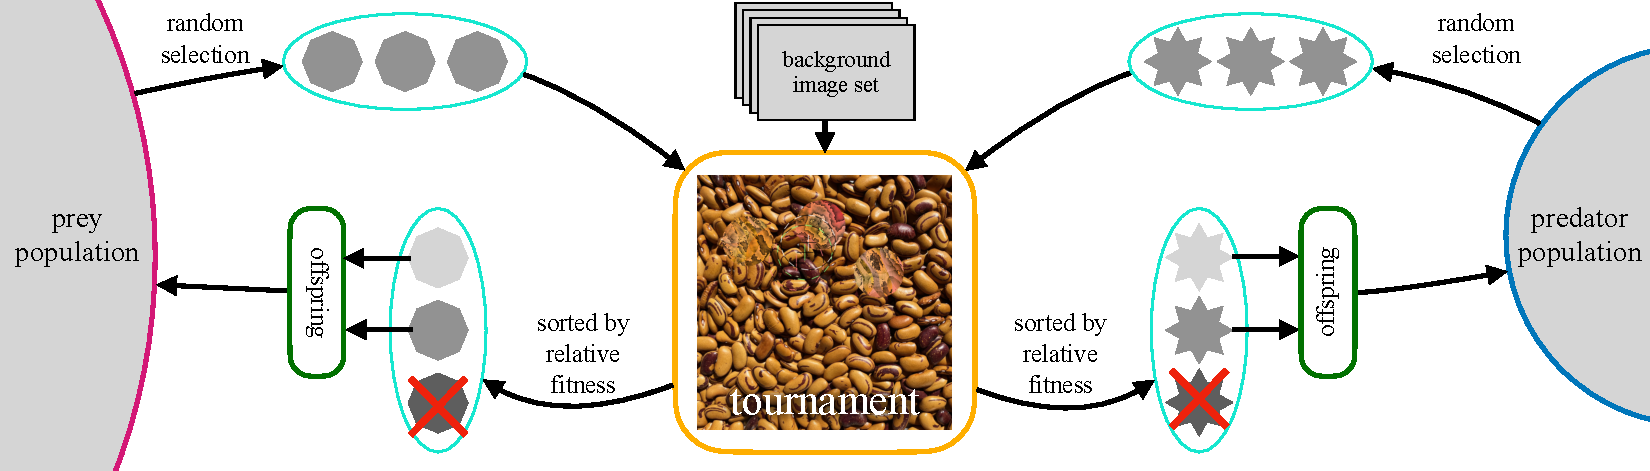
\includegraphics[width=\textwidth]{coc_overview.pdf}
    \caption{Overview of one step of the coevolutionary simulation of camouflage. Three prey are selected at random from their population of 200. Similarly for three predators from their population of 20. A random background image is selected from the given set, and a random crop of 512² pixels is made. The three prey are rendered to random non-overlapping locations. This composite image is given to each predator which estimates a position (circled crosshairs in tournament image, see also Figure \ref{fig:predator_responses}) predicting the center point of the most conspicuous prey. The predators are scored by “aim error” — the distance from their estimate to the \jargon{ground truth} center of the nearest prey. If the best predator's estimate is \textit{inside} a prey's disk, that prey is eaten and replaced by a new offspring of the other two prey. If the worst scoring predator's estimate is \textit{outside} all prey, it may die of starvation, to be replaced by a new offspring.}
    \Description{Overview diagram of the coevolutionary simulation of camouflage evolution.}
    \label{fig:simulation_overview}
\end{figure*}

%%%%%%%%%%%%%%%%%%%%%%%%%%%%%%%%%%%%%%%%%%%%%%%%%%%%%%%%%%%%%%%%%%%%%%%%%%%

\section{Related Work}
This work builds on \citet{reynolds_iec_2011} by replacing the human predator there with an evolving population of procedural predators, which \jargon{hunt} using a learning vision model. An earlier attempt at this approach, using coevolution and procedural predators, was described by \citet{harrington_coevolution_2014}.
\par
Closely related work on learning surface textures to camouflage 3D objects within real 3D scenes is described in \citet{owens_camouflaging_2014} for cubes, using one technique, and in \citet{guo_ganmouflage_2022}, for arbitrarily shaped 3D objects, using an improved technique. In both cases, the 3D scene is described by a set of photos from various viewpoints. The textures mapped onto the object to be camouflaged must trade off being inconspicuous from all viewpoints in the scene.
\par
Other computer graphics work related to camouflage include meticulously detailed reproduction of coloration patterns on real animals \cite{de_gomensoro_malheiros_leopard_2020} and generation of visual puzzles incorporating camouflaged images \cite{chu_camo_image_2010} \cite{Zhang_Yin_Nie_Zheng_2020}. CamoEvo \cite{hancock_camoevo_2022} is a toolbox for authoring online camouflage evolution games to understand evolution in real biological species. Being web-based, such simulations can be powered by very large numbers of human volunteers — citizen scientists — an instance of \jargon{human-based computation}.
\par
This adversarial coevolutionary simulation has clear similarities to \jargon{generative adversarial networks} (GANs) originally described in \citet{goodfellow_gan_2014}. Observer-driven optimization of camouflage patterns is a natural application of GANs, as in CamoGAN \cite{talas_camogan_2020}. However the goal of the current work (as suggested in the Future Work section of \citet{reynolds_iec_2011}) is to produce a simulation of a natural system, suitable for “what if” experiments which cannot be performed in the natural world.
\par
The procedural texture synthesis used here to generate camouflage patterns has a long history. This work is perhaps most directly inspired by \citet{perlin_image_1985} where images are rendered from purely procedural representation of 3D textures. A recent example of this approach is found in \citet{Guerrero_MatFormer_2022}. The combination of texture synthesis under control of a genetic algorithm goes back to \citet{sims_artificial_1991}, which in turn was inspired by the interactive biomorph evolution demo in \citet{dawkins_blind_1986}. FormSynth \cite{latham_form_1989} inspired Mutator \cite{todd_evolutionary_1994} and other tools.
\par
Evolution is represented in this model using \jargon{genetic programming} (GP), a population-based evolutionary optimization algorithm. It was first described by \citet{cramer_representation_1985} and popularized by \citet{koza_genetic_1992}. GP is a variation of \jargon{genetic algorithms} (GA). GA traditionally use a fixed length bit string as its genetic representation, while GP uses an arbitrarily-sized tree-shaped representation. GP trees conveniently map onto nested expressions in a domain specific language. Texture synthesis in this work is based on nested expressions of texture operators from the \texsyn{} library, see Figure \ref{fig:TexSyn_overview}. A prey population of these textures is optimized for camouflage effectiveness by GP using the selection pressure from a population of predators which determine fitness. \texsyn{} is used with the \jargon{strongly typed} variant of Genetic Programming known as STGP \cite{montana_strongly_1995}, one of several grammar-based GP variants \cite{Mckay_2010}. The GP implementation used here is called \lazypredator{}.
\par
The biological literature on camouflage and related topics is vast. A few starting points include: an early survey of camouflage in nature, \citet{thayer_concealing-coloration_1909}, pioneering work on mathematical models of biological patterns \citet{turing_chemical_1952}, revisiting Turing's work with modern computation \citet{murray_how_1988}, and a modern perspective on how life evolves and learns in \citet{valiant_probably_2013}.
\par

%%%%%%%%%%%%%%%%%%%%%%%%%%%%%%%%%%%%%%%%%%%%%%%%%%%%%%%%%%%%%%%%%%%%%%%%%%%

\subsection{Camouflaged Object Detection (COD)}
The last several years has seen a surge of computer vision research on \jargon{camouflaged object detection} — a part of predator behavior — finding camouflaged objects. (See for example this well-curated publication list: \citet{visionxiang_cod}.) COD systems seek to \jargon{segment} camouflaged objects in images: identify the pixels they cover. A recent example, which surveys this topic and presents its own strong solution, is \citet{Zhang2022}. Other research on COD include some based on boundaries \cite{chen_boundary-guided_2022} \cite{sun_boundary-guided_2022}, a mixed-scale approach \cite{pang_zoom_2022}, one based on transformer architecture \cite{yin_camoformer_2022}, and an attempt to rank camouflaged objects by “conspicuousness” \cite{lv_cod_2022}.
\par
COD attempts \textit{a priori} camouflage “breaking” — detecting the presence of well camouflaged objects — without learning either the background or the typical appearance of prey camouflage found in a given environment. That is, they are \jargon{generalist} predators, effectively using a form of \jargon{salience}. As summarized in \citet{Zhang2022}, COD is based on several labeled datasets (CHAMELEON, CAMO, and COD10K) carefully annotated by hand at the pixel level.
\par
In contrast, the goal of the simulation reported in this paper is to pit camouflage evolution against vision-based hunting. So determining the exact (pixel level) shape of the prey is largely irrelevant. This simulation ignores segmentation, abstracting prey as a disk of constant size, so sufficiently characterized by its center position. A real world predator can aim its attack at a prey's center without an exact segmentation. This work needs to find the \textbf{most} conspicuous prey, not all of them. This work simulates predators learning to find prey despite evolving camouflage patterns. Thus this model \jargon{adapts} to dynamic camouflage rather than approach COD as a static task of generalist detection. Significantly, this work requires no hand-labeled datasets at all, since it uses a form of \jargon{self-supervision}.
\par

%%%%%%%%%%%%%%%%%%%%%%%%%%%%%%%%%%%%%%%%%%%%%%%%%%%%%%%%%%%%%%%%%%%%%%%%%%%

\begin{figure*}
    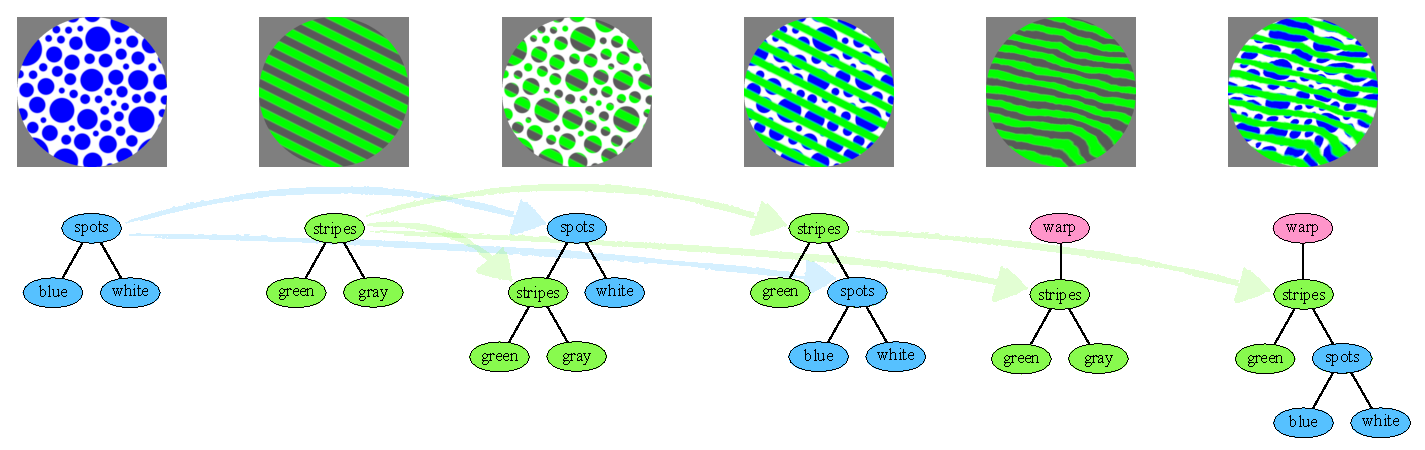
\includegraphics[width=\textwidth]{texsyn_overview.pdf}
    \caption{\texsyn{} expression trees and crossover between them, using a simplified version of \texsyn{} with three texture operators (\texttt{spots}, \texttt{stripes}, and \texttt{warp}) plus four named solid color textures. Minimal operator trees are shown in (a) and (b). \textit{Crossover} between (a) and (b) is shown in (c) and (d). (c) is \texttt{spots} where \texttt{blue} is replaced with \texttt{stripes}. (d) is \texttt{stripes} where \texttt{gray} is replaced with \texttt{spots}. (e) and (f) show (c) and (d) under a \texttt{warp} operator. (See Supplemental Material for actual \texsyn{} c++ code used for these examples.)}
    \Description{Overview of \texsyn{} representation of texture and the idea of \textit{crossover} between expression trees.}
    \label{fig:TexSyn_overview}
\end{figure*}

%% maybe more detail about GP and TexSyn in appendix? I think that does not add to page count

%%%%%%%%%%%%%%%%%%%%%%%%%%%%%%%%%%%%%%%%%%%%%%%%%%%%%%%%%%%%%%%%%%%%%%%%%%%

\section{Components of the Simulation}
\subsection{Coevolution, Populations, and Fitness}
This camouflage simulation is based on two adversarial \jargon{populations}: one of \jargon{predators} and one of \jargon{prey}. Individual prey compete for survival within their own population, similarly for predators. Predators must \jargon{hunt} successfully to “eat” and so survive. Prey survive if inconspicuous (cryptic) enough to avoid being found and eaten. Prey that is hunted and eaten, or a predator perished from hunger, is removed from its population. It is replaced by an \jargon{offspring} of parents from the surviving population.
\par
Predators define the fitness of prey: being easy to spot is bad, blending in is good. Similarly prey define the fitness of predators: being fooled by camouflage is bad, spotting cryptic prey is good. From this adversarial interaction, the two populations \jargon{coevolve}. If one side has some sort of flaw, the other side is motivated to exploit it. As a result both sides tend to improve over simulated time.
\par
Initial random prey have coloration likely to contrast with the background. Initial predators have a \jargon{pre-trained} ability to find conspicuous (salient) objects which often allow them to hunt these initially un-camouflaged prey. As coevolution proceeds, prey become better camouflaged against the given background images. In parallel, predators become more attuned to hunting these prey on the given backgrounds.
\par

%%%%%%%%%%%%%%%%%%%%%%%%%%%%%%%%%%%%%%%%%%%%%%%%%%%%%%%%%%%%%%%%%%%%%%%%%%%

\subsection{Tournaments, Competition, Relative Fitness}
\label{subsec:tournaments}
It is common in \jargon{evolutionary computation} to define \jargon{fitness} as a function that maps an \jargon{individual} (of the evolving population) into a number. That is, the function somehow evaluates the individual and assigns it a score. Typically this fitness function is \jargon{idempotent}: its value depends only on static properties of the given individual. This can be seen as \jargon{absolute fitness}.
\par
In contrast, this simulation uses \jargon{relative fitness}, determined by \jargon{competition} between individuals, in \jargon{tournaments}. A tournament is a game — a contest — between multiple individuals. 
\par
A simple example of relative fitness is a foot race. The winner of the race is the first to cross the finish line. The order of finishing \jargon{sorts} the racers by speed. Races have been run this way since ancient times. Today it is simple to precisely measure each runner's speed but that is not required to determine who won the race. Now consider two people playing chess. We do not know how to measure or predicts a player's skill. But by pitting them against each other, having them play a game (or a series of games) the results provide a useful measurement of relative fitness. 
\par
Throughout this model, \textbf{tournaments involve three individuals}. (Unlike the simulation in \citet{reynolds_iec_2011} which used tournaments of 10.) One simulation step (see Figure \ref{fig:simulation_overview}) consists of drawing three prey individuals out of their population to compete in a tournament. Like a foot race, or chess game, a tournament serves to sort the individuals according to relative fitness. That relative fitness results from the behavior of adversarial predators. During the same simulation step, three predators are drawn from their population. Each predator looks at the same input: an image with three camouflaged prey overlaid on a background image. The predators compete with each other for accurate hunting of the prey. The prey compete with each other by hiding (not being found) by the predators.
\par

%%%%%%%%%%%%%%%%%%%%%%%%%%%%%%%%%%%%%%%%%%%%%%%%%%%%%%%%%%%%%%%%%%%%%%%%%%%

\subsection{Negative Selection, Drift, and Mixability}

A modern synthesis \cite{livnat_sex_2016} of evolution theory, game theory, and machine learning (the multiplicative weights update algorithm: “no-regret learning”) suggests evolution may act to optimize \jargon{mixability}, a type of modularity in the genetic representation of phenotypes. As described in \citet{chastain_multiplicative_2013} this perspective focuses on the “...special case of weak selection in which all fitness values are assumed to be close to one another. ...hypothesizing that evolution proceeds for the most part not by substantial increases in fitness but by essentially random drift...” This concept goes back to the “Neutral Theory” in \citet{kimura_evolutionary_1968}.
\par
The evolutionary model used in the current work, implemented in software called \jargon{\lazypredator{},} attempts to operate in this “neutral” mode. Genetic algorithms often seek to promote the population's highest fitness individuals. They allow these high fitness individuals to survive longer and reproduce more often. This \jargon{elitism} can skew the evolutionary search: too much \jargon{exploiting} without enough \jargon{exploring.}  In contrast, \lazypredator{} uses \textit{negative selection} to encourage \jargon{drift}. Higher fitness individuals experience almost no difference in  relative fitness. It is the lowest fitness individuals that get culled by predation. In each tournament (see section \ref{subsec:tournaments}) the goal is to sort the three individuals by relative fitness. In fact, the only requirement is to identify the \textbf{least fit} of the three individuals.
\par 
For example, a predator looks at a scene then predicts the location of the most conspicuous of three prey. If this location is within the disk-shaped “body” of a prey, it is the \textbf{least} fit of the prey tournament and gets “eaten.” The relative fitness ordering of the other two prey is not significant and is ignored. If all predators \jargon{fail} and predict positions outside all three prey, then the entire simulation step is abandoned, no prey is eaten, and the prey population is unchanged.
\par
In the predator population, a tournament is ranked by the \textbf{distance from a predator's prediction to the center of the nearest prey} — essentially the predator's “aiming error.” The worst predator might then die from \jargon{starvation} based on its recent history of hunting success: has it eaten enough to survive? Currently this threshold is 40\% hunting success over its last 20 attempts.

%%%%%%%%%%%%%%%%%%%%%%%%%%%%%%%%%%%%%%%%%%%%%%%%%%%%%%%%%%%%%%%%%%%%%%%%%%%

\subsection{Offspring, Crossover, and Mutation}
In the prey population, a tournament is used to find the lowest relative fitness. This corresponds to the worst camouflage, the \jargon{most conspicuous} of three prey in a tournament. If a predator successfully locates a prey, we assume it is captured and eaten. The object representing that departed prey is removed from its population and replaced with a new individual. This is the \jargon{population update} stage of a steady-state genetic programming system \cite{syswerda_study_1991}.
\par
The new prey, which replaces the one killed by predator, is called the \jargon{offspring} of two other prey. This is the motivation for using tournaments of size 3: the least fit prey dies, and is replaced by the offspring of the tournament's two surviving prey. This is why their relative fitness is irrelevant, they both become the \jargon{parents} given as input to the \jargon{crossover} operation.
\par
In GP (and \lazypredator{}) individuals are represented as tree structures. In this simulation, those trees are interpreted as \texsyn{} programs as described in Section \ref{subsec:texture_synthesis}. The crossover operation is defined on two abstract trees. The two parents are first copied to preserve them. One copy is chosen as recipient and one as donor. In each a “random subtree” is selected. The recipient's random subtree is replaced by the donor's random subtree, by splicing the pointers between tree nodes. This is shown in Figure \ref{fig:TexSyn_overview}.
\par
After crossover, a mutation operator further modifies the offspring tree. It traverses the tree, finding all the leaf nodes, which here correspond to numerical constants in the texture programs. Because \lazypredator{} uses \jargon{strongly typed genetic programming} \cite{montana_strongly_1995} each leaf belongs to a specific user defined type (for example: a floating point number between 0 and 1). A method of the type's class can mutate (“jiggle”) the constant value of a leaf node (for example, add a small signed random offset, then clip back into the type's range). After crossover and mutation the new offspring is inserted into the population, replacing the dead prey.
\par

%%%%%%%%%%%%%%%%%%%%%%%%%%%%%%%%%%%%%%%%%%%%%%%%%%%%%%%%%%%%%%%%%%%%%%%%%%%
%% prototyping CNN diagram

\begin{figure}
    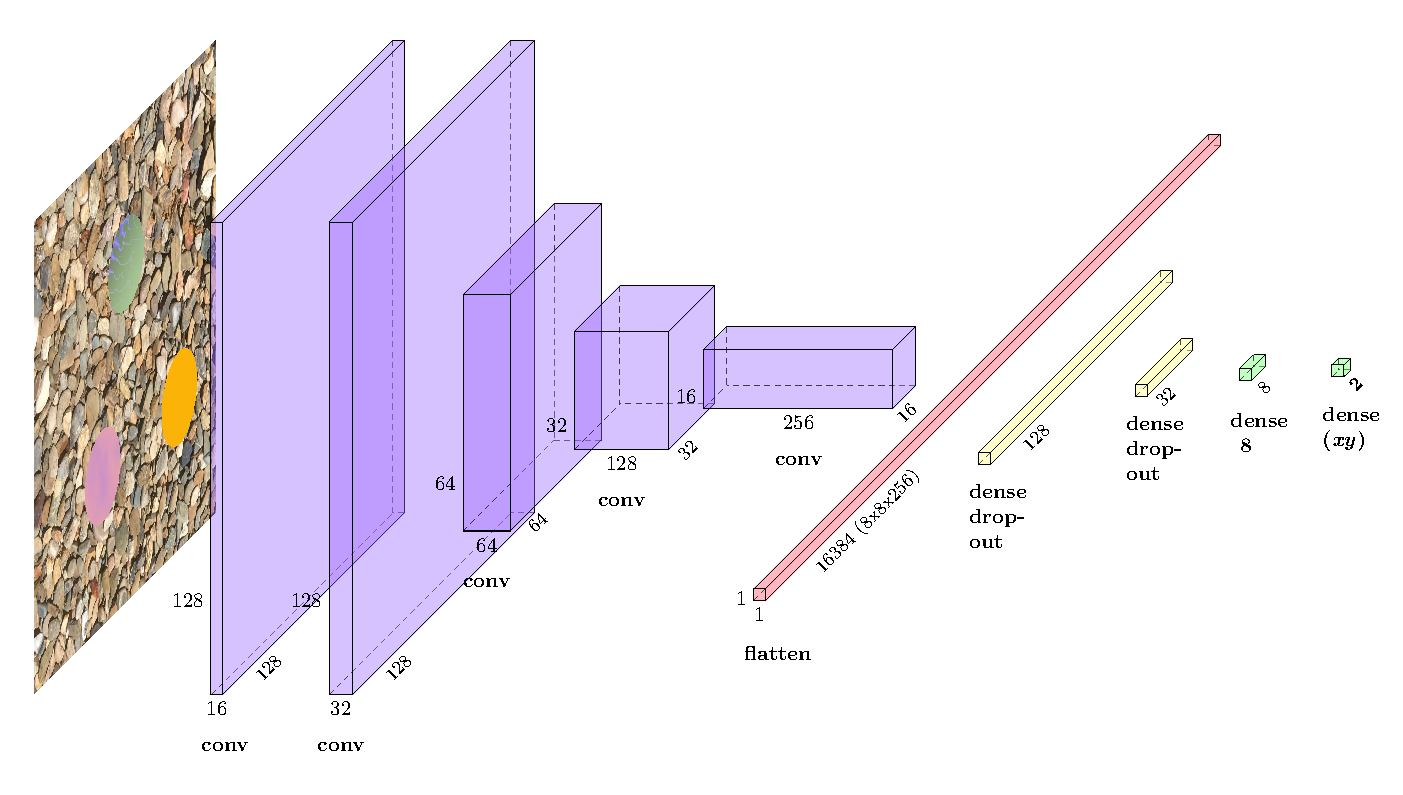
\includegraphics[width=\columnwidth]{predator_cnn.pdf}
    \caption{Architecture of a predator's neural net which maps a 128² RGB image into an \textit{xy} location where it estimates the most conspicuous prey is centered. All convolution layers but the first use strides of (2,2) while doubling the number of learned filters. Then fully connected layers reduce the flattened features, by factors of 4, down to an output layer of 2 values. This model contains 3.2 million parameters (More details in Supplemental Materials.)}
    \Description{Diagram of Predator's convolutional neural net.}
    \label{fig:predator_cnn}
\end{figure}

%%%%%%%%%%%%%%%%%%%%%%%%%%%%%%%%%%%%%%%%%%%%%%%%%%%%%%%%%%%%%%%%%%%%%%%%%%%
%% Full step/tournament image with predator responses

\begin{figure}
    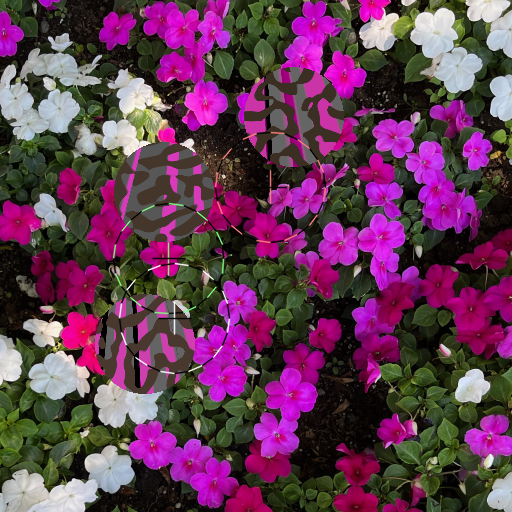
\includegraphics[width=\columnwidth]{20221007_0806_step_7030.png}
    \caption{Tournament image after simulation step. Starts with crop from given background set. Composited over that are three prey with evolved camouflage patterns. Over that are drawn three \jargon{crosshair} marks showing the responses of three predators. These are ranked by minimum distance to a prey center. Best is in black and white, second best is green and black, third is red and black. Here, only the top ranked predator chose a position inside a prey's disk, the other two failed. Choice of prey, predators, background image, crop, and prey placement — are all uniform random selection.}
    \Description{Full tournament image showing background, three prey, and three predator responses.}
    \label{fig:predator_responses}
\end{figure}


%%%%%%%%%%%%%%%%%%%%%%%%%%%%%%%%%%%%%%%%%%%%%%%%%%%%%%%%%%%%%%%%%%%%%%%%%%%

\subsection{Texture Synthesis}
\label{subsec:texture_synthesis}
Textures are represented in this simulation as trees of procedural texture operators. These correspond directly to nested expressions in a typical programming language. \jargon{\texsyn{}} is a simple domain specific language for describing textures.
\par
The details of \texsyn{} are not central to understanding this camouflage model. A quick overview is given here. \texsyn{} is library, an API, with many \jargon{operators} each of which return a \jargon{Texture}. Most of them also take Textures as input parameters, along with simple values like colors, 2d vectors, and scalars (floating point numbers). Writing nested functional expressions of \texsyn{} operators corresponds to trees of operator instances.
\par
These \texsyn{} textures are represented by operators, trees, and parameters. They do not store pixel data. Instead the Texture class provides a function to sample the texture's color at an arbitrary floating point \textit{xy} location. That color is computed on the fly. This is similar to GPU \jargon{fragment shaders} and the Pixel Stream Editor functions in \citet{perlin_image_1985}. Figure \ref{fig:TexSyn_overview} shows some simple examples and how these textures can be recombined with tree crossover.
\par
Note that the images in this paper are rendered at 512² pixels and the prey disks have a diameter of 100 pixels. These images are downsampled to 128² for use by predator's vision CNNs.
\par

%%%%%%%%%%%%%%%%%%%%%%%%%%%%%%%%%%%%%%%%%%%%%%%%%%%%%%%%%%%%%%%%%%%%%%%%%%%

\subsection{Predator Vision}
It is the predator's job to look at a tournament image and “hunt” for prey. These images are built from a portion of a background photo and overlaid with three randomly placed camouflaged prey. The camouflage texture for each disk shaped prey is rendered on the \texsyn{} side. Because all images in this simulation are synthetic, they are labeled with the random \jargon{ground truth} position data for each prey. This allows predators to learn in a \jargon{self-supervised} manner.
\par
\subsubsection{Pre-Training Predator's Vision}
\label{sec:pre_train_predator}
The basis for a predator's visual system is \textbf{a \jargon{pre-trained} deep neural net model for a “find conspicuous disk” task}, see Figure \ref{fig:predator_cnn}. The goal of this task is to look at an arbitrary image and locate the centerpoint of the most conspicuous (salient) region, assumed to be a prey-sized disk. This pre-training is done once then reused for each subsequent camouflage evolution run. \texsyn{} was used to generate a dataset of 20,000 labeled training examples called \jargon{FCD5}. (Effective training set size via augmentation was 500,000.) Each example was an RGB image, a 128×128×3 tensor, with an associated label: an \textit{xy} coordinate pair indicating a location in the image.
\par
Each training image starts with a \jargon{random texture} or a random crop of a photo (from a library of background images, see Section \ref{subsec:background_sets}). Over it was rendered one or three prey disks with random texture. While “random texture” is a slippery concept, the meaning here is the sort of prey texture used to initialize the prey population before an evolution run. The \lazypredator{} genetic programming engine has facilities for creating random trees of a given size from a user-defined \jargon{function set} such as one corresponding to the \texsyn{} library. A random tree is interpreted as a random nested expression of \texsyn{} operators with randomly chosen leaf constants. As such these prey textures are quite varied, but have a fair amount of structure, they are not uncorrelated noise. See, for example, Figure \ref{fig:time_sequence} (leftmost image) and Figure \ref{fig:fcd5_examples}.
\par
Each image in the “find conspicuous disk” training dataset is generated in one of three styles chosen with equal probability. Style 1 has a single prey disk, and the label is its center point. Style 2 has three different prey. Style 3 has three copies of a single prey disk. The latter two cases reduce the visibility of two of the three disks, by blending or dithering the pixels of the prey disk into the background. The label corresponds to the disk whose visibility is not reduced, presumed to be more conspicuous. See Figure \ref{fig:fcd5_examples}.
\par
\subsubsection{Fine-Tuning Predator's Vision}
During simulations of camouflage evolution, each predator is initialized as a copy of the pre-trained “find conspicuous disk” model to which noise is added. (Zero mean noise of less than 0.003 is added to each parameter of the deep neural net.) In each simulation step, the three predators chosen to participate in the tournament (see Figure \ref{fig:simulation_overview}) predict a prey position. Then \textbf{each predator is \jargon{fine-tuned} based on a dataset of labeled images collected during this simulation run}. This dataset is a collection of images from earlier simulation steps in this run. It is essentially the memory of prey coloration recently found in this environment. The fine-tuning dataset starts empty, then collects each tournament image until the dataset holds 500 images. Thereafter, each new tournament image replaces one of the 500 chosen at random. Labels for this dataset correspond to predictions made by the “best” predator (least aim error) in each step, see Figure \ref{fig:predator_responses}.
\par

%%%%%%%%%%%%%%%%%%%%%%%%%%%%%%%%%%%%%%%%%%%%%%%%%%%%%%%%%%%%%%%%%%%%%%%%%%%

\subsection{Background Sets}
\label{subsec:background_sets}
Each simulation run is based on a \jargon{background set} of images, usually photographs of natural scenes. These images form the background of tournament images, over which the camouflaged prey are drawn. These background images play the role of an \jargon{environment} in which prey need to hide to avoid being found and eaten by predators. Because the model is purely 2d, photographs offer an easy way to provide a variety of environments, of plausible natural complexity, in which to test camouflage evolution.
\par
Background sets used in this work consist of from 1 to 14 photographs, most have 4 or 5 photos. Almost all are casual snapshots taken with a mobile phone. The images in a background set are all similar. For example a set called \texttt{oak\_leaf\_litter} has six images, all of slightly different portions of leaves fallen on the ground. Each image in this set is taken with the camera pointing straight down, all from about the same height. As a result the images have features (e.g. leaves) of about the same size. This “similarity” helps the camouflage evolution process by providing many unique yet consistent backgrounds in which to try hiding.
\par
As used here, “similarity” is meant to suggest image features have a \jargon{stationary distribution}, that different patches have the same statistical distribution of color and frequency. When background sets are “less stationary” it becomes \jargon{harder} for evolution to find good camouflage. See discussion of limitations in Section \ref{subsec:limitations}.

\par

%%%%%%%%%%%%%%%%%%%%%%%%%%%%%%%%%%%%%%%%%%%%%%%%%%%%%%%%%%%%%%%%%%%%%%%%%%%

\subsection{Simulation Runs}
To run this coevolutionary simulation model, two processes are launched. One is the evolutionary texture synthesis system that models a population of prey with camouflage, it is c++ code based on \texsyn{} and \lazypredator{}. The other is a “predator server” that manages a population of visual hunters and fine-tunes their visual perception. This \predatoreye{} is Python code using Keras \cite{chollet_keras_2015} and TensorFlow \cite{tensorflow_whitepaper_2015}. The prey side produces a labeled tournament image. It is inspected by the predator side, which sends back a target location within the image, indicating its estimate of where the most conspicuous prey is. The labeled tournament image is used to fine-tune the predators. The target location drives the fitness function for prey evolution.
\par
The parameters for a simulation run are primarily a choice of background set (see section \ref{subsec:background_sets}), a scale factor for the background images, and a seed for random number generation. There are a few other parameters to the \texsyn{} command. These and other key parameters are summarized in Supplemental Materials.
\par
A typical run consists of 6000 steps with a prey population of 200 and predator population of 20. A preliminary version, reimplementing the interactive approach of \citet{reynolds_iec_2011}, used a prey population of 120 and typical runs of 2000 to 3000 steps. This was also typical for an intermediate version using a single pre-trained predator. The introduction of a population of predators reduced the rate of fine-tuning of predator's neural net models, leading to the longer 6000 step simulations.
\par
During a simulation run various data is collected in log files. The most important output is a “visual log” — periodically saving tournament images (a crop of the given backgrounds overlaid with camouflaged prey, as in Figure \ref{fig:teaser}) along with the predator response data. These images are saved “occasionally.” Originally it was every 20 steps, but was changed to every 19 steps to be relatively prime and so cycle through the 6 or 10 \jargon{subpopulations} (\jargon{demes} or \jargon{islands}) of the prey population.
\par

%%%%%%%%%%%%%%%%%%%%%%%%%%%%%%%%%%%%%%%%%%%%%%%%%%%%%%%%%%%%%%%%%%%%%%%%%%%

\section{Discussion}
This simulation model was applied to a variety of background sets to produce prey camouflage patterns suited to those environments. Figures \ref{fig:jans_oak_leaves_4x} to \ref{fig:michaels_gravel_4x} shows examples from several runs. 
% remember to check those \ref{}s in case ordering change.
% (Many additional examples, and other details of the development of this model, can be found in the project diary, whose URL is hidden for purposes of double-blind review. [... can I say this? reconsider after response from papersadmin@siggraph.org ...])
\par
These experiments were run on a 2021 Apple MacBook Pro with an M1 Max chip. A typical recent simulation run showed the predator vision/learn process taking about “600\%” of the processing power (that is, about 6 of 10 cores) and the prey texture render/evolve process taking about 10\% of a core (many steps use previously rendered prey). The time to complete a single simulation step is about 10 seconds. Typical runs are 6000 steps, so 60,000 seconds, about 16 hours. (Somewhat less since it takes 500 steps for the fine-tuning dataset to reach full size.) Unfortunately there is a bug in the \jargon{TensorFlow-Metal plug-in layer} which prevents this TensorFlow-based code from running on the GPU. When the bug is fixed, the overall simulation might run about 10 times faster, but that remains to be seen.
\par
A key observation from these experiments is that different background sets have differing degrees of difficulty. For some background sets, a simulated evolution run produces effective camouflage. Occasionally it is effective enough to momentarily fool a human observer: “Wait, where is the third prey?!” In other cases, runs (even repeated runs) fail to produce good results. So far this difference cannot be reliably predicted nor addressed. Anecdotally, it seems the more “stationary” the background textures are (see Section \ref{subsec:background_sets}) the easier it is to evolve effective camouflage.
% [... See blog entry: \href{https://cwreynolds.github.io/TexSyn/#20220930}{Reliability: what \textit{is} the likelihood of camouflage?} see also comment “Perhaps the common issue is large areas of nearly uniform [but contrasting] colors” in post \href{https://cwreynolds.github.io/TexSyn/#20221119}{Trouble with orange pyracantha}. I next did the elm(?) leaves and as expected that run went fine. Maybe the way to say it is that “easy” backgrounds are those where a correctly chosen uniform color can do a reasonable job of matching the backgrounds. See also comments in post \href{https://cwreynolds.github.io/TexSyn/#20221122}{Leaf litter by Plum, et al.}. — \textbf{Maybe this topic belongs in Discussion?} ...]
\par

%%%%%%%%%%%%%%%%%%%%%%%%%%%%%%%%%%%%%%%%%%%%%%%%%%%%%%%%%%%%%%%%%%%%%%%%%%%

\section{Limitations}
\label{subsec:limitations}
Chief among the limitations of this work is the lack of an objective measure of camouflage effectiveness. Without such a metric it is impossible to, for example, simply plot how camouflage effectiveness increases over simulated time. Without a metric it is hard to simply evaluate adjustments to the model: is a new parameter value better or worse?
\par
Another limitation is that all results are hand selected: “cherry picked.” After a simulation run, the resulting images are examined by a human who selects some as representative of the results, and makes a mental judgement of their effectiveness. From an objective standpoint, it is hard to claim that this simulation even “works.” Subjectively, it seems clear that it does: conspicuous prey seen early in a simulation tend to become less frequent, while cryptic prey become more common and effective (see Figure \ref{fig:time_sequence}).
\par
Other limitations include the inherently 2D nature of the simulation, that simulated time is discrete, and that the model of texture synthesis lacks genetic or biological plausibility. These are among the simplifying abstractions intended to make this initial model of camouflage coevolution tractable. But it is fair to complain that as a result, the model is \textit{too} abstract to provide much insight.
\par

%%%%%%%%%%%%%%%%%%%%%%%%%%%%%%%%%%%%%%%%%%%%%%%%%%%%%%%%%%%%%%%%%%%%%%%%%%%

\section{Future Work}
The goal of this work has been to build a computational model of the coevolution of camouflage from the interaction of predator and prey. Part of that was simply to show that camouflage can in fact arise from such a system. It also provides a simplistic automatic process to generate camouflage for a given environment from photos. The most important aspect of the work has been to create an open source model allowing future experiments, to help study camouflage in nature, and the perceptual phenomena of camouflage more generally.
\par
Section \ref{subsec:limitations} notes this model lacks an objective metric of camouflage effectiveness. One approach would be to take a \jargon{standard predator} (like one pre-trained on the FCD5 dataset, Section \ref{sec:pre_train_predator}) and testing it repeatedly against a given prey. The metric would be its average “miss” rate. Other work \cite{lv_cod_2022} suggests potential ways to rank “conspicuousness.” Where a candidate metric proposed, the model presented here would be a useful testbed for its evaluation. It should be possible to validate these candiddate metrics with crowd-sourced rating of camouflage quality, as in SEE Games \cite{stevens_games_2022} and CamoEvo \cite{hancock_camoevo_2022}.
\par
If an objective measure of camouflage quality did exist, many parameter settings of the current model could be revisited (see table in Supplemental Materials). For example, the size of predator and prey populations could be varied to find the best combination. Similarly: do much longer runs produce better quality?
\par
An important next step is to understand the failure modes of this simulation. Why some environments (background sets) are \textit{hard} while others are \textit{easy}? Why does this difference persist through repeated runs with differing random number seeds?
% As discussed in “\href{https://cwreynolds.github.io/TexSyn/#20221119}{Trouble with orange pyracantha}” and “\href{https://cwreynolds.github.io/TexSyn/#20221106}{Rerun kitchen granite}”.
Easy environments produce effective camouflage. Hard environments do not. They seem to move toward effective camouflage, then stop improving. Examining the “fossil record” of these runs, occasional isolated examples of effective camouflage do appear. For some reason they are lost to predation. They fail to reproduce so cannot spread through the population. That better camouflage \textit{is} discovered by prey evolution may suggest that the problem is not there but in the predators. How can certain (hard) background sets cause predators to “go off on a tangent”?
\par
In early versions, simulated predators often incorrectly predicted prey to be at the tournament image's center. Perhaps this \jargon{center preference} is a “lazy” default strategy, since that is the mean position over all prey positions. To work around this, random prey center placement was constrained to avoid positions within one prey diameter of the image center. This seems like a bug to be better understood and fixed in a more principled way.
\par
This simulation is currently a mixed paradigm model using both evolution and learning. While these typically co-occur in nature \cite{valiant_probably_2013}, it would be interesting to look at an all-evolution model with evolved detectors for predators, perhaps along the lines of \citet{bi_genetic_2022}. Or conversely, an all learning model, something similar to CamoGAN \cite{talas_camogan_2020}.
\par
An obvious next step is to apply this model to 3d environments. Perhaps along the lines described in \citet{miller_color_2022}. One key simplifying assumption of the current purely 2d model is that plausible, naturally complex, environments are provided by simple photographs from the phone in our pocket. Providing plausibly complex 3d environments will be much harder. Perhaps neural techniques like NeRF (e.g. \cite{gao_nerf_2022}) will meet that need.
\par

%%%%%%%%%%%%%%%%%%%%%%%%%%%%%%%%%%%%%%%%%%%%%%%%%%%%%%%%%%%%%%%%%%%%%%%%%%%

%% Acknowledgements
\begin{acks}
I deeply appreciate everyone who helped me with this work: my family for loving support, Ken Perlin for (well, lots, but especially) PSE \cite{perlin_image_1985}, Andrew Glassner for teaching me everything I know about deep learning \cite{glassner_deep_2021}, and Pat Hanrahan for some key career advice (“just do the research”).
\par
I've been working on this project on and off since 2007, based on inspirations by papers in the early 1990s (\citet{witkin_reaction_1991}, \citet{turk_generating_1991}, \citet{angeline_competitive_1993}, \citet{sims_artificial_1991}, and \citet{sims_evolving_1994}). Also one paper published a year before I was born: \citet{turing_chemical_1952}.
Thanks for additional help from:
Bilal Abbasi,
Jan Allbeck,
Rebecca Allen,
Richard Dawkins,
Steve DiPaola,
Aaron Hertzmann,
Bjoern Knafla,
John Koza,
Dominic Mallinson,
Nick Porcino,
and Michael Wahrman.
\par
Thanks also to my neighbors whose landscaping provided many of the background images used here.
\par
\end{acks}

%%%%%%%%%%%%%%%%%%%%%%%%%%%%%%%%%%%%%%%%%%%%%%%%%%%%%%%%%%%%%%%%%%%%%%%%%%%

%% Bibliography.
\newpage
\bibliographystyle{ACM-Reference-Format}
\bibliography{coc.bib}

%%%%%%%%%%%%%%%%%%%%%%%%%%%%%%%%%%%%%%%%%%%%%%%%%%%%%%%%%%%%%%%%%%%%%%%%%%%

%% two "figure only" pages can be included at the end of the paper.

\begin{figure*}
    \igfour{20221228_step_6662.png}
    \hfill
    \igfour{20221228_step_7095.png}
    \hfill
    \igfour{20221228_step_7574.png}
    \hfill
    \igfour{20221228_step_7742.png}
    \caption{Four tournament images from run jans\_oak\_leaves\_20221227\_1717.}
    \Description{QQQ.}
    \label{fig:jans_oak_leaves_4x}
\end{figure*}

\begin{figure*}
    \igfour{20221108_2018_step_4655.png}
    \hfill
    \igfour{20221108_2018_step_5498.png}
    \hfill
    \igfour{20221108_2018_step_5947.png}
    \hfill
    \igfour{20221108_2018_step_6562.png}
    \caption{Four tournament images from run tree\_leaf\_blossom\_sky\_20221108\_2018.}
    \Description{QQQ.}
    \label{fig:tree_leaf_blossom_sky_4x}
\end{figure*}

\begin{figure*}
    \igfour{20221121_1819_step_6324.png}
    \hfill
    \igfour{20221121_1819_step_6464.png}
    \hfill
    \igfour{20221121_1819_step_6677.png}
    \hfill
    \igfour{20221121_1819_step_6755.png}
    \caption{Four tournament images from run plum\_leaf\_litter\_20221121\_1819.}
    \Description{QQQ.}
    \label{fig:plum_leaf_litter_4x}
\end{figure*}

\begin{figure*}
    \igfour{20221112_1555_step_6495.png}
    \hfill
    \igfour{20221112_1555_step_5510.png}
    \hfill
    \igfour{20221112_1555_step_5681.png}
    \hfill
    \igfour{20221112_1555_step_6370.png}
    \caption{Four tournament images from run rock\_wall\_20221112\_1555.}
    \Description{QQQ.}
    \label{fig:rock_wall_4x}
\end{figure*}

\begin{figure*}
    \igfour{20221218_step_5396.png}
    \hfill
    \igfour{20221218_step_5641.png}
    \hfill
    \igfour{20221218_step_5947.png}
    \hfill
    \igfour{20221218_step_6753.png}
    \caption{Four tournament images from run yellow\_flower\_on\_green\_20221217\_1826.}
    \Description{QQQ.}
    \label{fig:yellow_flower_4x}
\end{figure*}

\begin{figure*}
    \igfour{20221215_step_5867.png}
    \hfill
    \igfour{20221215_step_5892.png}
    \hfill
    \igfour{20221215_step_6830.png}
    \hfill
    \igfour{20221215_step_6916.png}
    \caption{Four tournament images from run michaels\_gravel\_20221214\_1837.}
    \Description{QQQ.}
    \label{fig:michaels_gravel_4x}
\end{figure*}

\begin{figure*}
    \ignine{20220303_UVSfqCzewt_38_20.png}
    \hfill
    \ignine{20220303_SBWaLRHOzk_56_33.png}
    \hfill
    \ignine{20220303_bUMqcbutgJ_25_78.png}
    \hfill
    \ignine{20220303_HZzUzWWqcC_54_28.png}
    \hfill
    \ignine{20220303_inuPKUxnHQ_72_71.png}
    \hfill
    \ignine{20220303_RRGCwhmcJc_101_84.png}
    \hfill
    \ignine{20220303_PYinyJAWaj_61_60.png}
    \hfill
    \ignine{20220303_TNXfhQtzYa_92_91.png}
    \hfill
    \ignine{20220303_cDMtFaTYKk_63_54.png}
    \\
    \vspace{0.1cm}
    \ignine{20220303_wIRPERwSCh_49_63.png}
    \hfill
    \ignine{20220303_edDsCjbHdf_61_92.png}
    \hfill
    \ignine{20220303_fGMFBgMQDX_93_86.png}
    \hfill
    \ignine{20220303_jQREPLQyuL_33_39.png}
    \hfill
    \ignine{20220303_ijBOHTccYX_104_101.png}
    \hfill
    \ignine{20220303_KAoOFAqFyU_80_58.png}
    \hfill
    \ignine{20220303_NExMwxEbzU_85_92.png}
    \hfill
    \ignine{20220303_kpcUyhHXOh_91_98.png}
    \hfill
    \ignine{20220303_oWPwPGkcSb_82_22.png}
    \\
    \vspace{0.1cm}
    \ignine{20220303_uAEPxMZbeo_83_45.png}
    \hfill
    \ignine{20220303_cADfBauZUV_47_32.png}
    \hfill
    \ignine{20220303_YAMfudJxeH_30_84.png}
    \hfill
    \ignine{20220303_JeyBgDfMcN_40_82.png}
    \hfill
    \ignine{20220303_OaOJaByhbU_90_55.png}
    \hfill
    \ignine{20220303_mhYpDjxaKf_78_57.png}
    \hfill
    \ignine{20220303_ASsEgFUlly_23_60.png}
    \hfill
    \ignine{20220303_nzgItDrYqT_71_99.png}
    \hfill
    \ignine{20220303_QuHYtnPora_72_73.png}
    \caption{Examples of the three types of labeled training example in the FCD5 training dataset for “find conspicuous disk” pre-training. \textbf{Top row, type 1}: single random prey over random background. \textbf{Middle row, type 2}: three different prey. \textbf{Bottom row, type 3}: three copies of one prey. For types 2 and 3, one prey is unaltered, the other two are blended into background, by differing amounts, to make them more muted, less conspicuous. See Section \ref{sec:pre_train_predator}.}
    \Description{Full tournament image showing background, three prey, and three predator responses.}
    \label{fig:fcd5_examples}
\end{figure*}

%%%%%%%%%%%%%%%%%%%%%%%%%%%%%%%%%%%%%%%%%%%%%%%%%%%%%%%%%%%%%%%%%%%%%%%%%%%

%% Appendix -- must become separate PDF document before submission.
\appendix
\onecolumn
\section{Supplemental Materials}
\subsection{Key Simulation Parameters}
\setcounter{page}{0}
\begin{minipage}{\linewidth}
The most fully detailed description of this simulation model is the source code of its reference implementation \textbf{(Note to reviewers: open source code will be made available if paper is accepted for publication)}. This table summarizes some of the key parameters which are used for all results shown in this paper.
\par

\begin{table}[H]
\begin{adjustwidth}{1cm}{0cm}
\begin{tabular}{ |l|r|r| }
\hline
\textbf{Parameter} & \textbf{value} & \textbf{x-large} \\ 
\hline
predator population & 20 & 40 \\ 
prey population & 200 & 400 \\ 
prey subpopulations (demes) & 10 & 20 \\
prey max init tree size & 100 & \\
prey min tree size after crossover & 50 & \\
prey max tree size after crossover & 150 & \\
\hline
prey render diameter (pixels) & 100 & \\ 
tournament output image size & 512×512 & \\ 
predator input image size & 128×128 & \\ 
\hline
tournament image save frequency & 19 & \\
simulation steps per run (typical) & 6000 & 12,000 \\
prey generation equiv (steps/pop) & 30 & \\
predator fail rate (typical) & 15\%-30\% & \\
predator starvation threshold & & \\
\hspace{0.2cm}(success in previous 20 attempts) & < 40\% & \\ 
\hline
predator “FCD” pre-training: & & \\
\hspace{0.2cm} synthetic dataset size & 20,000 & \\
\hspace{0.2cm} effective size with augmentation & 500,000 & \\
\hline
max signed “jiggle” noise added to  & & \\
\hspace{0.2cm} all params of new predator CNN & 0.003 & \\
\hline
\end{tabular}
\end{adjustwidth}
\label{table:key_simulation_parameters}
\end{table}
\end{minipage}

\subsection{Background Image Sets}
\begin{minipage}{\linewidth}
Names and descriptions for the sets of background images used in this paper, see section \ref{subsec:background_sets}. Each set is composed of several photographs of a similar natural scene. \textbf{(Note to reviewers, these images can be made available, along with source code, other data and development documentation.)}
\par
\begin{table}[H]
\begin{adjustwidth}{1cm}{0cm}
\begin{tabular}{ |l|l|c|c| }
\hline
\textbf{name} & \textbf{description} & \textbf{photos} & \textbf{figures} \\ 
\hline
backyard\_oak &
    under canopy of “California live oak” &
    12 & \ref{fig:backyard_oak_4x} \\
\hline
bean\_soup\_mix &
    mixture of dried beans &
    4 & \ref{fig:bean_soup_mix_4x} \\
\hline
jans\_oak\_leaves &
    (white?) oak leaf litter (by Jan Allbeck in Fairfax, Virginia) &
    6 & \ref{fig:jans_oak_leaves_4x} \\
\hline
kitchen\_granite &
    polished granite counter-top in our kitchen &
    6 & \ref{fig:kitchen_granite_4x} \\
\hline
mbta\_flowers &
    flowers (impatiens?) near MBTA Northeastern stop &
    4 & \ref{fig:predator_responses}, \ref{fig:mbta_flowers_4x} \\
\hline
michaels\_gravel &
    gravel bed in neighbor’s front yard &
    4 & \ref{fig:teaser}, \ref{fig:predator_cnn}, \ref{fig:michaels_gravel_4x} \\
\hline
oak\_leaf\_litter &
    fallen oak leaves on edge of road &
    6 & \ref{fig:time_sequence} \\
\hline
oxalis\_sprouts &
    sprouts of Oxalis push through leaf litter after first rain &
    5 & \ref{fig:teaser} \\
\hline
plum\_leaf\_litter &
    fallen leaves from plum and other trees, near sunset &
    5 & \ref{fig:teaser}, \ref{fig:plum_leaf_litter_4x} \\
\hline
rock\_wall &
    “dry stack” retaining wall in a neighbor's front yard &
    14 & \ref{fig:rock_wall_4x} \\
\hline
tiger\_eye\_beans &
    dried heirloom “tiger eye” beans from farmers market  &
    5 & \ref{fig:simulation_overview} \\
\hline
tree\_leaf\_blossom\_sky &
    small trees (branches, leaves, and blossoms) sky background &
    5 & \ref{fig:teaser}, \ref{fig:tree_leaf_blossom_sky_4x} \\
\hline
yellow\_flower\_on\_green &
    “Scot's broom” or “French broom” in neighbor's yard &
    6 & \ref{fig:yellow_flower_4x} \\
\hline

\end{tabular}
\end{adjustwidth}
\label{table:background_sets}
\end{table}
\end{minipage}

\subsection{\texsyn{} \texttt{c++} Code for Figure \ref{fig:TexSyn_overview}}
% Better to use listings package?  https://ctan.org/pkg/listings
\begin{minipage}{\linewidth}
\begin{adjustwidth}{1cm}{0cm}
\begin{small}
\begin{verbatim}
Uniform white(1);
Uniform gray(0.1);
Uniform blue(0, 0, 1);
Uniform green(0, 1, 0);
LotsOfSpots spots(0.9, 0.05, 0.3, 0.02, 0.02, blue, white);
Grating stripes(Vec2(), green, Vec2(0.1, 0.2), gray, 0.3, 0.5);
NoiseWarp warp_stripes(1, 0.1, 0.7, stripes);
LotsOfSpots spots2(0.9, 0.05, 0.3, 0.02, 0.02, stripes, white);
Grating stripes2(Vec2(), green, Vec2(0.1, 0.2), spots, 0.3, 0.5);
NoiseWarp warp_all(1, 0.1, 0.7, stripes2);
\end{verbatim}
\end{small}
\end{adjustwidth}
\end{minipage}

% Note (from https://s2022.siggraph.org/technical-papers-submissions-faq/): 
% The Conference Paper track encourages submissions for high-quality, 
% ground-breaking research that fits within a strict 7-page limit (plus 
% additional pages for references), and may be more appropriate for
% research that is less-polished but still potentially-impactful. Journal 
% papers do not have a page limit, and may include more thorough experiments
% and derivations within the main paper. 


\subsection{Additional Parameters to Simulation Runs}
\begin{minipage}{\linewidth}
Command line arguments to pkgT:
\par
\begin{adjustwidth}{1cm}{0cm}
\begin{small}
\begin{verbatim}
pkgT requires at least one pathname parameter, others may be omitted from the end:
    background image directory (required)
    output directory (defaults to .)
    background scale (defaults to 0.5)
    random seed (else: default seed)
    window width (defaults to 1200)
    window height (defaults to 800)
    individuals (defaults to 120)
    subpopulations (defaults to 6)
    max init tree size (defaults to 100)
    min crossover tree size (default max init tree size  * 0.5)
    max crossover tree size (default max init tree size  * 1.5)
\end{verbatim}
\end{small}
\end{adjustwidth}
\end{minipage}

\subsection{Details of Pre-Trained Predator Model}
\begin{minipage}{\linewidth}
The pre-trained predator visual system, shown in Fig. \ref{fig:predator_cnn}, is a Keras TensorFlow CNN model with about 3.2 million parameters. Its input is a 128×128 pixel RGB image and its output is an \textit{xy} location where it estimates the most conspicuous prey is centered. \textbf{(Note to reviewers: the data for this pre-trained model will be made available if paper is accepted for publication)}. Here is its \texttt{model.summary()}:
\par
\begin{adjustwidth}{1cm}{0cm}
\begin{small}
\begin{verbatim}

Model: "sequential"
_________________________________________________________________
 Layer (type)                Output Shape              Param #
=================================================================
 conv2d (Conv2D)             (None, 128, 128, 16)      1216
 dropout (Dropout)           (None, 128, 128, 16)      0
 conv2d_1 (Conv2D)           (None, 64, 64, 32)        12832
 dropout_1 (Dropout)         (None, 64, 64, 32)        0
 conv2d_2 (Conv2D)           (None, 32, 32, 64)        51264
 dropout_2 (Dropout)         (None, 32, 32, 64)        0
 conv2d_3 (Conv2D)           (None, 16, 16, 128)       204928
 dropout_3 (Dropout)         (None, 16, 16, 128)       0
 conv2d_4 (Conv2D)           (None, 8, 8, 256)         819456
 dropout_4 (Dropout)         (None, 8, 8, 256)         0
 flatten (Flatten)           (None, 16384)             0
 dense (Dense)               (None, 128)               2097280
 dropout_5 (Dropout)         (None, 128)               0
 dense_1 (Dense)             (None, 32)                4128
 dense_2 (Dense)             (None, 8)                 264
 dense_3 (Dense)             (None, 2)                 18
=================================================================
Total params: 3,191,386
Trainable params: 3,191,386
Non-trainable params: 0
\end{verbatim}
\end{small}
\end{adjustwidth}
\end{minipage}
\par

\subsection{Additional Samples of Simulation Runs}

\begin{figure}[H]
    \igfour{20230101_step_10561.png}
    \hfill
    \igfour{20230101_step_10750.png}
    \hfill
    \igfour{20230101_step_10950.png}
    \hfill
    \igfour{20230101_step_11861.png}
    \caption{Four tournament images from run bean\_soup\_mix\_20221231\_1317.}
    \Description{QQQ.}
    \label{fig:bean_soup_mix_4x}
\end{figure}

\begin{figure}[H]
    \igfour{20230106_step_11019.png}
    \hfill
    \igfour{20230106_step_11204.png}
    \hfill
    \igfour{20230106_step_11689.png}
    \hfill
    \igfour{20230106_step_11995.png}
    \caption{Four tournament images from run mbta\_flowers\_20230105\_1114.}
    \Description{QQQ.}
    \label{fig:mbta_flowers_4x}
\end{figure}

\begin{figure}[H]
    \igfour{20230111_step_5576.png}
    \hfill
    \igfour{20230111_step_6159.png}
    \hfill
    \igfour{20230111_step_6303.png}
    \hfill
    \igfour{20230111_step_6726.png}
    \caption{Four tournament images from run kitchen\_granite\_20230110\_1758.}
    \Description{QQQ.}
    \label{fig:kitchen_granite_4x}
\end{figure}

\begin{figure}[H]
    \igfour{20230115_step_6902.png}
    \hfill
    \igfour{20230115_step_7682.png}
    \hfill
    \igfour{20230115_step_7942.png}
    \hfill
    \igfour{20230115_step_12413.png}
    \caption{Four tournament images from run backyard\_oak\_20230113\_2254.}
    \Description{QQQ.}
    \label{fig:backyard_oak_4x}
\end{figure}

%%%%%%%%%%%%%%%%%%%%%%%%%%%%%%%%%%%%%%%%%%%%%%%%%%%%%%%%%%%%%%%%%%%%%%%%%%%

\end{document}